\documentclass[../dissertation.tex]{subfiles}

\begin{document}

\subsection{Experiment 4 - WiFi Connection}

Experiment 4 investigates the effect of using a WiFi network connection for message passing experiments. The target robot car platform described in Section \ref{background-robot-config} utilise a WiFi connection, thus understanding the effect this will have on the communication performance is required to understand the final performance of the system.

It is also reasonable that multi-robot systems may desire each robot to be physically mobile, thus a wired network connection may not be feasible in many set-ups. It is important to understand how this technology will affect perforrmance compared to the ideal wired situation.

The Raspberry Pi 3 Model B's utilised in these experiments contain 802.11n WiFi chips which support a 2.4GHz network connection.

The experiment consists of running the same code in both a wired (Ethernet) situation and a wireless (WiFi) situation. As before, the code will send timestamped messages from the sender host to the echoer host, which will send it back to the sender. The sender then records the message id and sent and received times to file. The code is run several times with a range of message frequencies from 200Hz to 2000Hz in 200Hz steps (200Hz, 400Hz, 600Hz, ...).

The hypothesis was that switching to WiFi would increase message latencies across all frequencies, and also reduce the maximum frequency that message latency remains consistent across the entire message stream (as in the previous experiment described in Section \ref{experiment3-cpu-speed}).

\subsubsection{Results}

The experimental results after 3 runs in each setup appeared to somewhat agree with the hypothesis. Overall message latency was higher across all frequencies using WiFi except 2000Hz - as shown in Figure \ref{exp4-means-all-freq}.

\begin{figure}[H]
\centering
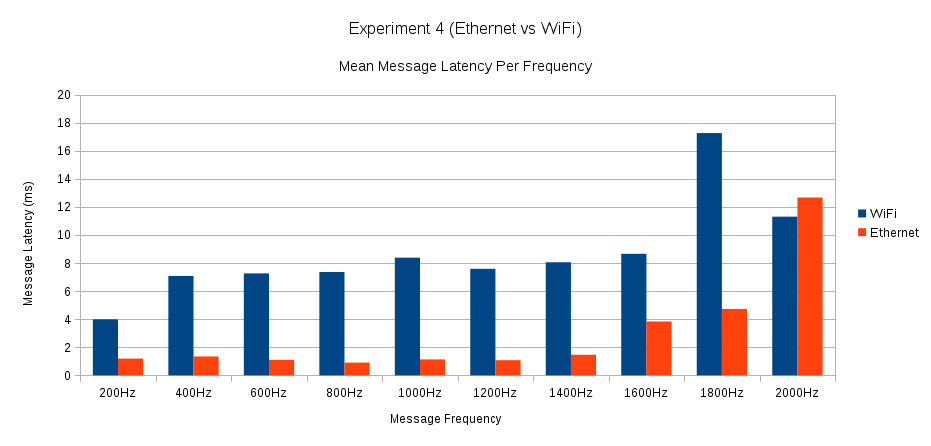
\includegraphics[width=\textwidth]{images/experiment4/mean_per_frequency.png}
\caption{Experiment 4 - Ethernet, All Frequencies}
\label{exp4-means-all-freq}
\end{figure}

Figures \ref{exp4-ethernet-all-freq} and \ref{exp4-wifi-all-freq} demonstrate averages across 3 runs for all frequencies of the message streams, for Ethernet and WiFi respectively. It is clear from these figures that WiFi gives even more erratic results than Ethernet, and thus it's effects must be carefully considered if using WiFi in future experiments.

\begin{figure}[H]
\centering
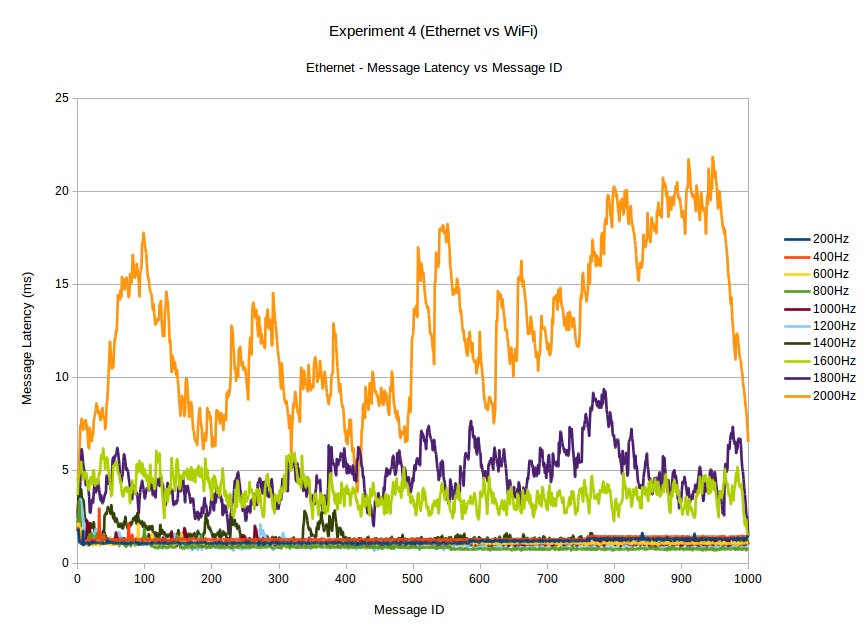
\includegraphics[width=\textwidth]{images/experiment4/ethernet_mean_times_pretty.png}
\caption{Experiment 4 - Ethernet, All Frequencies}
\label{exp4-ethernet-all-freq}
\end{figure}

\begin{figure}[H]
\centering
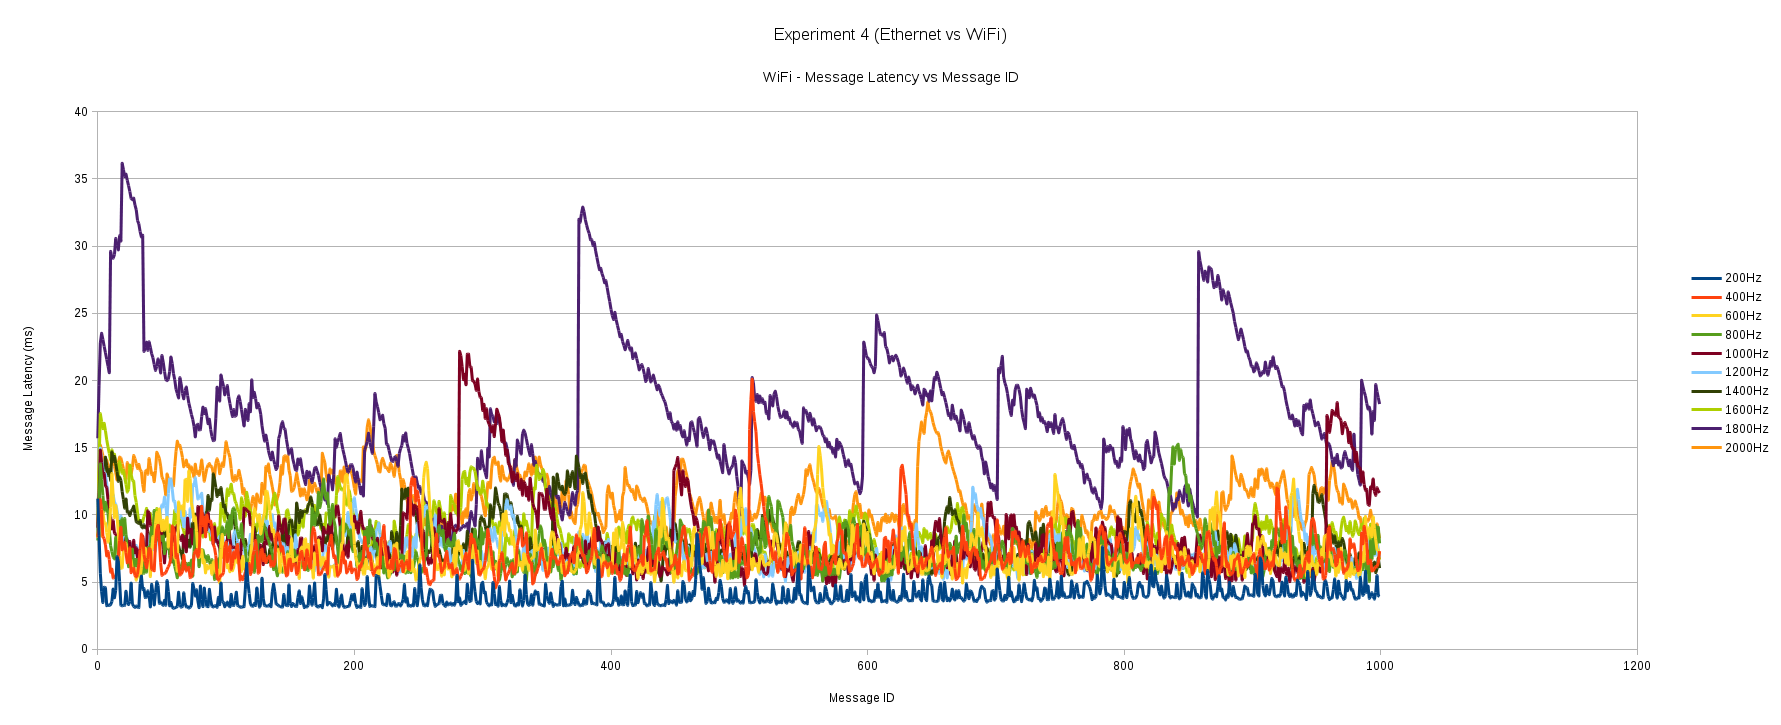
\includegraphics[width=\textwidth]{images/experiment4/wifi_mean_times_pretty.png}
\caption{Experiment 4 - WiFi, All Frequencies}
\label{exp4-wifi-all-freq}
\end{figure}

\end{document}
